\chapter{Sprints}
Bei einem Sprint handelt es sich um einen kurzen und festdefinierten Zeitraum, in welchem ein Team eine bestimmte Menge an Aufgaben erledigt. In der Regel umfasst dieser Zeitraum bis zu 30 Tage. Dabei haben die Sprints in einem Team immer dieselbe Länge. Sprints sind ein wesentlicher Bestandteil von Scrum und bieten eine Möglichkeit, schnell auf Änderungen zu reagieren.\cite{Wolf2021-ef} Während der Entwicklung dieser Anwendung beträgt die Sprintdauer zwei Wochen.
\section{Erster Sprint der dritten Veröffentlichung}
Die Bearbeitungsphase des ersten Sprints verläuft vom 19.06.2023 bis zum 02.07.2023.
Da am Ende der zweiten Veröffentlichung erneut Zeitmangel herrschte, um eine qualitativ hochwertige Anwendung zu liefern, wird erneut versucht aufwendige Storys und Aufgaben in den ersten Sprint zu legen. Dadurch soll mehr Zeit für die Qualitätssicherung im zweiten Sprint zur Verfügung stehen.
\subsection{User Storys}
Die User Storys stellen eine vom Nutzer mögliche Aktion mit einer Ausgangssituation, der jeweiligen Aktion für die User Story und einer Endsituation dar. Im Folgenden werden die User Storys des ersten Sprints des dritten Releases beschrieben und es wird gegebenfalls bei einer starken Abweichung zwischen der benötigten Zeit und der geschätzten Zeit der jeweiligen Story begründet, warum die geschätzte Zeit nicht für die Umsetzung der User Story ausreichend war. Eine Auflistung aller User Storys mit der jeweiligen benötigten Zeit und der jeweiligen geschätzten Zeit ist in der Tabelle~\ref{tab:story} zu finden. 
\subsubsection{Beschreibung der Storys}

Im Folgenden werden die Storys beschrieben. Dabei wird es auf die erzielte beziehungsweise gewünschte Funktionalität eingegangen, die durch eine Aktion des Nutzers erfolgt.

\textbf{\hyperlink{T216}{\hypertarget{S216}{STP23M-216}}: Start a dialog with NPC}

Durch diese Story wird die Funktionalität des Dialogsystems übergangsweise implementiert. Somit kann der Nutzer mit einem beliebigen NPC-Trainer mittels der Interaktionstaste einen Dialog starten. Die Dialogstexte werden von dem Team Magical Studios bereitgestellt und entsprechend in die angebotenen Sprachen übersetzt.

\textbf{\hyperlink{T217}{\hypertarget{S217}{STP23M-217}}: Close Dialog with NPC}

Der laufende Dialog mit dem NPC-Trainer soll mit dieser Story beendet werden können, um das Spiel fortzusetzen. Dabei muss das Ende des Dialogs erreicht werden, um den Dialog beenden zu können. 

\textbf{\hyperlink{T218}{\hypertarget{S218}{STP23M-218}}: Next Dialog with NPC}

Diese Story ermöglicht es dem Nutzer, mit dem nächsten Dialogabschnitt mit dem NPC-Trainer fortzufahren. Es werden dabei möglicherweise Dialogoptionen beziehungsweise Fragen seitens des NPC-Trainers angezeigt, auf die der Nutzer beim Fortfahren reagieren soll.

\textbf{\hyperlink{T219}{\hypertarget{S219}{STP23M-219}}: Starter Monsters Popup}

Der Nutzer interagiert mit dem NPC-Trainer für Starter-Monster in einem geöffneten Dialogfenster. Nach Drücken der Interaktionstaste öffnet sich ein Popup, das Starter-Monster in einer Karussellansicht mit kurzen Beschreibungen und Attributen zeigt.

\textbf{\hyperlink{T220}{\hypertarget{S220}{STP23M-220}}: Choose Starter Monster}

Das Popup für die Auswahl der Starter-Monster wird angezeigt. Der Nutzer wählt ein beliebiges Monster aus und das Popup schließt sich daraufhin. Es öffnet sich ein neues Popup, in dem das gewählte Monster dargestellt wird.

\textbf{\hyperlink{T221}{\hypertarget{S221}{STP23M-221}}: Close Monster Received Popup}

Durch diese Story kann der Nutzer einen weiteren Dialogabschnitt von dem NPC-Trainer für Starter-Monster sehen, wenn der Nutzer das Popup des Erhalts des Starter-Monsters schließt. 

\textbf{\hyperlink{T222}{\hypertarget{S222}{STP23M-222}}: Starter Monster already Received}

Mit dieser Story erhält der Nutzer einen Dialogabschnitt von dem NPC-Trainer für Starter-Monster, dass der Nutzer bereits Starter-Monster erhalten hat. Dies erfolgt, sobald der Nutzer mit dem NPC-Trainer für Starter-Monster interagiert und bereits Starter-Monster besitzt.

\textbf{\hyperlink{T223}{\hypertarget{S223}{STP23M-223}}: Start an Encounter with a Trainer}

Ziel dieser Story ist es, einen Kampf mit einem (NPC-)Trainer zu starten. Dabei wird ein Dialog mit dem Trainer gestartet, um die Kampfszene einzuleiten. Es erfolgt beim Abschließen des Dialogs eine Ankündigung für den Nutzer, dass der Kampf in Kürze gestartet wird.

\textbf{\hyperlink{T224}{\hypertarget{S224}{STP23M-224}}: Switch to Encounter Scene Trainer}

Der Nutzer sieht die Ankündigung, dass der Kampf in Kürze gestartet wird. Der Nutzer bestätigt die Ankündigung mit der Interaktionstaste und die Szene wechselt daraufhin zum Kampfbildschirm. In diesem Fall ist der Kampf ein Kampf gegen einen (NPC-)Trainer.

\textbf{\hyperlink{T227}{\hypertarget{S227}{STP23M-227}}: Heal Monsters Popup}

Nachdem der Nutzer mit der Krankenschwester durch einen Dialog interagiert hat, öffnet sich ein Bestätigungsfenster für das Heilen der Monster. Der Nutzer kann sich entscheiden, mit dem Heilen der Monster fortzufahren oder das Heilen zu verweigern.

\textbf{\hyperlink{T228}{\hypertarget{S228}{STP23M-228}}: Heal Monsters}

Durch diese Story kann der Nutzer seine Monster heilen. Der Nutzer sieht das Bestätigungsfenster und bestätigt die Aktion. Daraufhin wird der Dialog mit der Krankenschwester fortgesetzt.

\textbf{\hyperlink{T229}{\hypertarget{S229}{STP23M-229}}: Refuse Heal Monsters}

Der Nutzer sieht das Bestätigungsfenster für die Aktion des Heilens. Dabei kann der Nutzer das Heilen der Monster verweigern. Die Krankenschwester antwortet in dem Dialog entsprechend. 

\textbf{\hyperlink{T230}{\hypertarget{S230}{STP23M-230}}: Start a dialog with Nurse}

Das Dialogsystem wird mit dieser Story erweitert, sodass der Nutzer spezielle Interaktionsdialoge beim Sprechen mit einer Krankenschwester erhält. Der Nutzer kann somit mit einer Krankenschwester beim Drücken der Interaktionstaste einen Dialog starten, wenn sie voreinander stehen.

\textbf{\hyperlink{T231}{\hypertarget{S231}{STP23M-231}}: Start a dialog with NPC Encounter}

Durch diese Story wird es dem Nutzer ermöglicht, mit anderen Trainern zu kämpfen. Der Kampf kann dann begonnen werden, sobald der Nutzer mit einem Trainer einen Dialog gestartet hat. Dabei werden bei NPC-Trainern Beispielsdialoge vor dem Kampf eingeblendet.

\textbf{\hyperlink{T232}{\hypertarget{S232}{STP23M-232}}: Start a dialog with NPC Starter Monster}

Der Erhalt des Starter-Monsters erfolgt mit dieser Story. Der Nutzer beginnt einen Dialog mit dem NPC-Trainer für Starter-Monster, der dem Nutzer eine Auswahl an Starter-Monstern anbietet.

\textbf{\hyperlink{T234}{\hypertarget{S234}{STP23M-234}}: Show Abilities}

Der Nutzer befindet sich in der Kampfszene. Beim Drücken des 'Fähigkeiten'-Knopfs sieht der Nutzer die möglichen Fähigkeiten, die sein jetziges Monster anwenden kann.

\textbf{\hyperlink{T235}{\hypertarget{S235}{STP23M-235}}: Use an Ability}

Das Ziel dieser Story ist es, eine Fähigkeit des jetzigen Monsters anzuwenden. Dabei sieht der Nutzer die Leiste mit den vorhandenen Fähigkeiten des jetzigen Monster und drückt auf den Knopf eine Fähigkeit auf der Leiste. Es wird der Zug gesetzt und die Fähigkeit angewandt.

\textbf{\hyperlink{T251}{\hypertarget{S251}{STP23M-251}}: Show Pause Menu}

Der Nutzer befindet sich im Spielbildschirm und möchte beispielsweise das Spiel verlassen. Er drückt auf den Knopf des Pausemenüs, dann erscheint das Pausemenü, mit dem der Nutzer das Spiel verlassen kann.

\textbf{\hyperlink{T252}{\hypertarget{S252}{STP23M-252}}: Show Settings Menu}

Der Nutzer sieht das Pausemenü, mit welchem er auf das Einstellungsmenü navigieren kann. Der Nutzer drückt auf den Knopf 'Einstellungen', wodurch das Einstellungsmenü erscheint.

\textbf{\hyperlink{T253}{\hypertarget{S253}{STP23M-253}}: Show Audio Settings}

Durch diese Story kann der Nutzer auf die Toneinstellungen navigieren. Der Nutzer sieht das Einstellungsmenü und drückt auf die Toneinstellungen. Dann erscheint das Einstellungsfenster für den Ton.

\textbf{\hyperlink{T254}{\hypertarget{S254}{STP23M-254}}: Change Audio Volume}

Ziel dieser Story ist es, die Lautstärke des Tons zu verwalten. Der Nutzer sieht die Toneinstellungen inklusive des Schiebereglers. Er zieht den Regler nach rechts und reduziert dadurch die Lautstärke des Tons.

\textbf{\hyperlink{T255}{\hypertarget{S255}{STP23M-255}}: Close Audio Settings}

Durch diese Story kann der Nutzer das Einstellungsfenster für den Ton schließen. Dabei drückt der Nutzer auf Pfeilknopf und das Einstellungsmenü wird angezeigt.

\textbf{\hyperlink{T261}{\hypertarget{S261}{STP23M-261}}: Go Back from Settings}

Der Nutzer sieht das Einstellungsmenü und drückt dabei auf den Pfeilknopf. Es wird infolgedessen das Pausemenü angezeigt.

\textbf{\hyperlink{T262}{\hypertarget{S262}{STP23M-262}}: Show Trainer Settings}

Der aktuelle Bildschirm zeigt das Einstellungsmenü. Der Nutzer drückt dabei den Knopf für die Trainereinstellungen und das Fenster dafür wird entsprechend dargestellt.

\textbf{\hyperlink{T263}{\hypertarget{S263}{STP23M-263}}: Change Trainer Character}

Die Trainereinstellungen werden auf dem Bildschirm angezeigt. Der Nutzer aktualisiert den Charakter seines Trainers und drückt dabei den Aktualisierungsknopf. Hierdurch wird der Trainer aktualisiert.

\textbf{\hyperlink{T264}{\hypertarget{S264}{STP23M-264}}: Delete Trainer Popup}

Der Nutzer sieht die Trainereinstellungen und drückt darin auf den Knopf 'Löschen'. Es erscheint dann ein Popup, in dem der Prozess des Löschens vom Nutzer bestätigt werden soll.

\textbf{\hyperlink{T265}{\hypertarget{S265}{STP23M-265}}: Delete Trainer}

Das Popup für das Löschen des Trainers wird angezeigt. Der Nutzer bestätigt das Löschen und der Bildschirm wechselt zum Mainmenü mit einem Bestätigungstext.

\textbf{\hyperlink{T267}{\hypertarget{S267}{STP23M-267}}: New Ingame}

Der Nutzer erstellt einen neuen Trainer und steigt in das Spiel ein. Es erscheinen nach ein paar Sekunden neue Nachrichten auf dem futuristischen Handy, die für den Nutzer eine Hilfestellung darstellen. 

\textbf{\hyperlink{T268}{\hypertarget{S268}{STP23M-268}}: Show Notification Messages}

Der Spielbildschirm wird mit ungelesenen Nachrichten auf dem futuristischen Handy dargestellt. Der Nutzer drückt auf das Handy und die ungelesenen Nachrichten werden angezeigt.

\textbf{\hyperlink{T269}{\hypertarget{S269}{STP23M-269}}: Close Phone}

Durch diese Story kann der Nutzer das futuristische Handy schließen. Er drückt dabei auf den Knopf 'Schließen' und das Handy wird zur ursprünglichen Größe verwandelt. 

\textbf{\hyperlink{T270}{\hypertarget{S270}{STP23M-270}}: Notification After Starter Monster}

Diese Story ermöglicht es dem Nutzer eine Hilfestellung nach dem Erhalt des Starter-Monsters zu erhalten. Der Nutzer erhält das Starter-Monster und als Folge daraus werden neue Nachrichten an das futuristische Handy mit einer Hilfestellung verschickt.

\textbf{\hyperlink{T271}{\hypertarget{S271}{STP23M-271}}: Notification After Low Health Monsters}

Der Nutzer hat einen Kampf verlassen, nach dem seine Monster niedrige Lebenspunkte haben. Der Nutzer erhält auf dem futuristischen Handy neue Nachrichten, die den Nutzer auf die Krankenschwester in 'Moncenter' hinweisen.

\textbf{\hyperlink{T278}{\hypertarget{S278}{STP23M-278}}: Close Trainer Settings}

Mit dieser Story kann der Nutzer die geöffneten Trainereinstellungen schließen. Dabei drückt der Nutzer auf den Pfeilknopf und es wird das Einstellungsmenü angezeigt.
\subsubsection{Bewertung der Storys}

Im Folgenden werden die Storys bewertet, welche eine starke Abweichung zwischen der benötigten Zeit und der geschätzten Zeit aufweisen.

\textbf{\hyperlink{T216}{\hypertarget{S216}{STP23M-216}}: Start a dialog with NPC}

Diese Story wurde mit fünf Story Points geschätzt und beträgt somit fünf Stunden als geschätzte Zeit. Der Entwickler benötigte dafür allerdings sechs Stunden und 40 Minuten. Der Grundaufbau des Dialogs und die entsprechende Übersetzung in die angebotenen Sprachen haben länger als erwartet benötigt. Dafür sind die anderen Storys \hyperlink{T217}{\hypertarget{S217}{STP23M-217}} und \hyperlink{T218}{\hypertarget{S218}{STP23M-218}} besser ausgefallen, da die Grundstruktur bereits etabliert ist.

\textbf{\hyperlink{T220}{\hypertarget{S220}{STP23M-220}}: Choose Starter Monster}

Die Funktionalität des Erhalts des Starter-Monsters beträgt als Story drei Story Points und somit drei Stunden als geschätzte Zeit. Der Entwickler benötigte aber vier Stunden insgesamt für den Abschluss der Story. Dies hängt damit zusammen, dass die Serverkommunikation, das Verbinden zwischen dem Client und dem Server sowie das Fortsetzen des Dialogs sich schwieriger als erwartet dargestellt hat.

\textbf{\hyperlink{T223}{\hypertarget{S223}{STP23M-223}}: Start an Encounter with a Trainer}

Die Story hat einen Story Point und somit beträgt die geschätzte Zeit eine Stunde. Allerdings konnte diese Story während des ersten Sprints nicht erledigt werden, da die Recherche über benötigte Informationen aus der Serverdokumentation erforderlich war und der Sprintzeitraum bis dahin nicht ausgereicht hatte.

\textbf{\hyperlink{T224}{\hypertarget{S224}{STP23M-224}}: Switch to Encounter Scene Trainer}

Diese Story beträgt fünf Story Points und somit hat fünf Stunden als geschätzte Zeit. Die Story konnte nicht innerhalb der geschätzten Zeit erledigt werden, da der Entwickler Verständisprobleme mit dem Erhalt der Ereignisse aus dem Server für den Kampfstart hatte. Dadurch hat sich der Abschluss dieser Story wesentlich verzögert.

\textbf{\hyperlink{T228}{\hypertarget{S228}{STP23M-228}}: Heal Monsters}

Die Funktionalität der Heilung der Monsters wurde mit zwei Story Points und somit mit zwei Stunden geschätzt. Sie wurde aber innerhalb von fünf Minuten von dem Entwickler implementiert, da der Entwickler bereits Erfahrung mit dem Dialogsystem und den Serverabfragen hat.

\textbf{\hyperlink{T229}{\hypertarget{S229}{STP23M-229}}: Refuse Heal Monsters}

Das Verweigern der Heilung der Monsters wurde mit einem Story Point und mit einer Stunde geschätzt. Es wurde aber innerhalb von fünf Minuten von dem Entwickler implementiert, da der Entwickler bereits Erfahrung mit der Heilungsfunktionalität hat.

\textbf{\hyperlink{T231}{\hypertarget{S231}{STP23M-231}}: Start a dialog with NPC Encounter}

Diese Story wurde mit einem Story Point und einer Stunde geschätzt. Der Entwickler benötigte aber fünf Minuten zum Erledigen der Story, da er sich mit dem Dialogsystem auskennt und somit die Story schneller erledigen konnte.

\textbf{\hyperlink{T234}{\hypertarget{S234}{STP23M-234}}: Show Abilities}

Das Anzeigen der Fähigkeiten des eigenen Monsters hat als Story drei Story Points und wurde mit drei Stunden geschätzt. Aufgrund von fehlender Zeit in dem ersten Sprint und fehlender Struktur der Kampfszene konnte die Story nicht erledigt werden und wurde in den zweiten Sprint verschoben.

\textbf{\hyperlink{T235}{\hypertarget{S235}{STP23M-235}}: Use an Ability}

Diese Story wurde mit vier Story Points und somit mit vier Stunden geschätzt. Da das Anzeigen der Fähigkeiten nicht implementiert worden ist, konnte diese Aufgabe auch nicht erledigt werden. Die Story wurde deshalb in den zweiten Sprint verschoben. 

\textbf{\hyperlink{T251}{\hypertarget{S251}{STP23M-251}}: Show Pause Menu}

Die Story wurde mit einem Story Point und somit mit einer Stunde geschätzt. Der Entwickler hat aber für das Erledigen der Story sechs Stunden und 30 Minuten gebraucht. Da das Pausemenü neu entworfen wurde, hat der Entwickler mehr Zeit als erwartet benötigt, um das neue Design zu implementieren. 

\textbf{\hyperlink{T252}{\hypertarget{S252}{STP23M-252}}: Show Settings Menu}

Das Anzeigen des Einstellungsmenüs hat als Story zwei Story Points und beträgt als geschätzte Zeit zwei Stunden. Die Story wurde von dem Entwickler innerhalb von vier Stunden erledigt und somit mehr als geschätzt, da der Entwickler Verbesserungsvorschläge seitens des Scrum-Masters umgesetzt hatte.

\textbf{\hyperlink{T254}{\hypertarget{S254}{STP23M-254}}: Change Audio Volume}

Die Funktionalität des Schiebereglers in den Toneinstellungen hat als Story drei Story Points und wurde somit mit drei Stunden geschätzt. Der Entwickler hat für die Story eine Stunde verbraucht, da der Entwickler bereits Erfahrung mit den Toneinstellungen in Kombination mit dem Task \hyperlink{T357}{\hypertarget{S357}{STP23M-357}} hatte.

\textbf{\hyperlink{T263}{\hypertarget{S263}{STP23M-263}}: Change Trainer Character}

Diese Story wurde mit vier Story Points und somit mit vier Stunden geschätzt. Der Entwickler hat dafür zwei Stunden und 20 Minuten benötigt. Aufgrund von bereits bestehenden Erfahrungen mit den Charakteren und Trainereinstellungen hat der Entwickler die Story schneller als erwartet erledigt.

\textbf{\hyperlink{T264}{\hypertarget{S264}{STP23M-264}}: Delete Trainer Popup}

Die Story wurde mit einem Story Point und somit mit einer Stunde geschätzt. Der Entwickler hat für die Story dennoch zwei Stunden und 30 Minuten benötigt. Da in dieser Story auch ein neues Design für das Popup hinzugekommen ist, erfolgte das Erledigen der Story mit mehr Aufwand.

\textbf{\hyperlink{T267}{\hypertarget{S267}{STP23M-267}}: New Ingame}

Das Anzeigen des futuristischen Handys und der Glocke beim neuen Einstieg in das Spiel wurde als Story mit zwei Story Points und somit mit zwei Stunden geschätzt. Der Entwickler benötigte für die Story allerdings 40 Minuten, da er sich mit entwurfstechnischen Implementierungen gut auskennt.

\textbf{\hyperlink{T268}{\hypertarget{S268}{STP23M-268}}: Show Notification Messages}

Diese Story wurde mit fünf Story Points und mit fünf Stunden geschätzt. Der Entwickler konnte die Story in drei Stunden und 30 Minuten erledigen, da er die Grundstruktur des Handys in der Story \hyperlink{T267}{\hypertarget{S267}{STP23M-267}} etabliert hatte und sie in dieser Story mit der Funktionalität erweitert hat.

\textbf{\hyperlink{T269}{\hypertarget{S269}{STP23M-269}}: Close Phone}

Die Story wurde mit einem Story Point und mit einer Stunde geschätzt. Der Entwickler hat für das Erledigen der Story lediglich fünf Minuten benötigt, da er sich mit der Funktionalität des futuristischen Handys bereits auskennt.

\textbf{\hyperlink{T271}{\hypertarget{S271}{STP23M-271}}: Notification After Low Health Monsters}

Das Anzeigen von Hilfestellung nach dem Verlust eines Kampfs hat als Story zwei Story Points und wurde somit mit zwei Stunden geschätzt. Da der Kampf in diesem Sprint nicht vollständig implementiert werden konnte, wurde die Story in den zweiten Sprint verschoben.

\textbf{\hyperlink{T278}{\hypertarget{S278}{STP23M-278}}: Close Trainer Settings}

Diese Story wurde mit einem Story Point und mit einer Stunde geschätzt. Der Entwickler hat für die Story fünf Minuten benötigt, da er die betroffenen Ansichten selbst implementiert hat, da er darin bereits Erfahrungen hatte.
\subsection{Aufgaben und Bugs}
Der erste Sprint hat zusätzlich zu den Storys vier Aufgaben und einen Bug. Dabei werden teilweise technische Grundlagen geschaffen, die die gesamte Anwendung betreffen oder Teile der Anwendung verbessern sollen. Im Vergleich zur zweiten Veröffentlichung fällt die Anzahl der Aufgaben und die geschätzte Zeit dieser allerdings geringer aus. Eine Auflistung aller Aufgaben ist in der Tabelle \ref{tab:task1} zu finden.

\subsubsection{Beschreibung der Aufgaben und Bugs}
Im Folgenden werden sämtliche Aufgaben und Bugs des ersten Sprints beschrieben. Es wird dabei auf ihre Einzelheiten eingegangen.

\textbf{\hyperlink{T282}{\hypertarget{S282}{STP23M-282}}: Hinzugekommene Services erstellen und alte erweitern}
\newline
\newline
In dieser Aufgabe geht es um das Erweitern der Services. Dabei müssen neue Api-Services und Services entsprechend der Serverdokumentation angelegt werden. Des Weiteren müssen sämtliche neue \Gls{DTO} hinzugefügt werden. Zusätzlich müssen alle bereits vorhanden Services und DTOs auf Veränderungen überprüft werden und gegebenenfalls verändert werden.
\newline
\newline
\textbf{\hyperlink{T297}{\hypertarget{S297}{STP23M-297}}: Minimap Gebietsdetails}
\newline
\newline
In der zweiten Veröffentlichung gab es die Anforderung, eine Regionskarte in Form eine Minimap zu implementieren. Dabei sollte die Minimap auch Details wie den Regionsnamen, Gebäudedetails und Beschreibungen beinhalten. Die Details sind aus Zeitmangel nicht mehr hinzugefügt worden. Diese Aufgabe soll die fehlende Anforderung aus dem zweiten Release nachholen.
\newline
\newline
\textbf{\hyperlink{T357}{\hypertarget{S357}{STP23M-357}}: Audio hinzufügen}
\newline
\newline
Eines der Bonusfeatures, welches mit dem Kunden vereinbart worden ist, ist es, die Anwendung mit Musik auszustatten. In der Aufgabe STP23M-357 sollen die technischen Möglichkeiten für dieses Bonusfeature gelegt werden. Zusätzlich sollen auch schon Audiodateien in bestimmten Bildschirmen abgespielt werden. So soll es eine Musik für die Menüs vor dem Spiel selbst geben. Eine andere  Musik soll in der Willkommensequenz abgespielt werden. Im Spiel soll, je nach Situation, ebenfalls verschiedene Lieder abgespielt werden. So sollen die Städte, Räume, Routen und Kämpfe jeweils eine eigene Musik erhalten.
\newline
\newline
\textbf{\hyperlink{T418}{\hypertarget{S418}{STP23M-418}}: Maprendering und Spriteanimation überarbeiten}
\newline
\newline
Diese Aufgabe soll die Darstellung der Spielwelt und die Animation der Figuren überarbeiten. Diese ist nach dem zweiten Release noch suboptimal und macht Probleme. Demnach gibt es Verschiebungen zwischen dem Dargestellten und der tatsächlichen Lage der Figur, sodass begehbare Tiles nicht begehbar sind und umgekehrt. Diese Probleme sollen mit dieser Aufgabe behoben werden.
\newline
\newline
\textbf{\hyperlink{T433}{\hypertarget{S433}{STP23M-433}}: Interagieren funktioniert nicht}
\newline
\newline
Hierbei handelt es sich um ein Bugticket. Dieser Bug ist aufgetaucht, nachdem die Richtung, in der die NPCs schauen, korrigiert wurde. Nach der Korrektur ist es nicht mehr möglich, andere Trainer anzusprechen. Das Ziel dieses Bugtickets ist es nun dafür zu sorgen, dass das Ansprechen wieder möglich ist.

\subsubsection{Bewertung der Aufgaben und Bugs}
Nur eine der vier Aufgaben ist innerhalb der geschätzten Zeit abgeschlossen worden. Die Aufgabe \hyperlink{S357}{STP23M-357} hat dabei nur etwas mehr als die Hälfte der geschätzten Zeit benötigt. Dies ist darauf zurückzuführen, dass die Implementierung des Audioservices durch die vorhandene \textit{JavaFX-Media} Bibliothek einfacher als gedacht ist. Die anderen drei Aufgaben haben die geschätzte Zeit überschritten. Die Aufgabe \hyperlink{S282}{STP23M-282} hat dabei die geringste Abweichung. Die Abweichung ist darauf zurückzuführen, dass diese Aufgabe in der Veröffentlichung von einer anderen Person übernommen worden ist als in den beiden anderen Veröffentlichungen. Etwas mehr als das Doppelte der geschätzten Zeit hat die Aufgabe \hyperlink{S297}{STP23M-297} gedauert. Dabei hat das dynamische Rendern der Minimap und das Anzeigen der Orte länger als erwartet gedauert. Ungefähr das 2,5-fache der geschätzten Zeit, hat die Erledigung derAufgabe \hyperlink{S418}{STP23M-418} benötigt. Hier wurde zunächst ein \textit{\Gls{PoC}} Projekt erstellt, um eine neue Implementierung für die Spriteanimation und Kamerabewegung zu testen. Dies allein hat einen Tag und zwei Stunden gedauert, womit die geschätzte Zeit bereits aufgebraucht war. Die eigentliche Implementierung beziehungsweise Änderung hat dann nochmal zwei Tage gedauert. Zusätzlich zu den vier Aufgaben ist während des Sprints ein Bug dazugekommen, welches auch direkt bearbeitet wurde. Hier hat die geschätzte Zeit mit der benötigten Zeit übereingestimmt.\\
Zur Bewertung kann abschließend gesagt werden, dass die Aufgaben deutlich länger gedauert haben, als im Vorhinein geschätzt. Dies ist auf die oben beschriebenen Begründungen zurückzuführen. Trotz der Abweichungen sind die Aufgaben und Bugs zufriedenstellend abgeschlossen worden, da keine Aufgaben mit in den zweiten Sprint übernommen werden müssen.
\subsection{Bewertung des Sprints}
In diesem Sprint sind verschiedene Aspekte der Anwendung bearbeitet worden und es sind neue Features dazugekommen. Entsprechend wurde das Pausemenü überarbeitet und ein neues Einstellungsmenü hinzugefügt. Die Trainereinstellungen, welche nun über das Einstellungsmenü zu erreichen sind, wurden ebenfalls überarbeitet. Neu hinzugekommen sind hier ein Audioeinstellungspopup und der Button für die Tastatureinstellung. Ebenso wurden die Minimap und das Rendern und Animieren der Sprites überarbeitet. Die Minimap zeigt nun alle Anforderungen der zweiten Veröffentlichung an. Neu implementiert wurde das Dialogsystem inklusive Interaktionen mit NPCs wie zum Beispiel das Auswählen eines Startmonsters und das Heilen der eigenen Monster. Darüber hinaus wurden die Bonusfeatures Musik in der Anwendung und das Handyfeature, welches Hilfestellungen im Spiel bietet, neu implementiert. Zum Schluss wurde begonnen, den Kampfbildschirm zu implementieren.\\
\begin{figure}[H]
    \center
    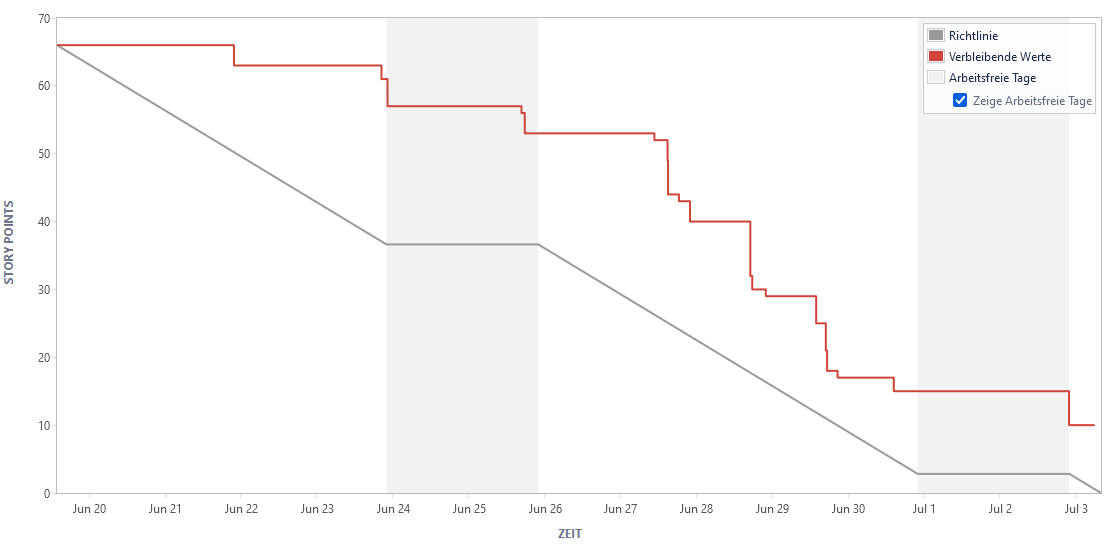
\includegraphics[height=0.5\textwidth]{images/burndown/sprint1Story.png}
    \caption{Burndown-Diagramm: Release 3: Sprint 1 Story Points}
    \label{fig: sprint1Story}
\end{figure}

Wie in Abbildung \ref{fig: sprint1Story} zu sehen ist, wurden nicht alle Storys abgeschlossen. Dies hat zwei Hauptursachen. Demnach wurden zu Beginn des Sprints nicht sehr viele Storys abgearbeitet. Dies wurde zwar versucht in der zweiten Woche wieder aufzuholen, was jedoch nicht komplett gelungen ist. Des Weiteren waren die Storys \hyperlink{S234}{STP23M-234} und \hyperlink{S235}{STP23M-235} von der Story \hyperlink{S224}{STP23M-224} geblockt, welche erst kurz vor Sprintende beendet wurden. Die Story \hyperlink{S271}{STP23M-271}, welche ebenfalls nicht abgeschlossen wurde, kann dabei erst implementiert werden, wenn ein Kampf beendet werden kann, da die Story davon abhängt. \\ Abschließend ist festzuhalten, dass der Sprint zufriedenstellend abgeschlossen wurde, auch wenn nicht alle Storys optimal ausgewählt worden sind.

\subsubsection{Erhöhung der Vorgänge}
Im ersten Sprint der dritten Veröffentlichung gab es eine Umfangsänderung.
\begin{figure}[H]
    \center
    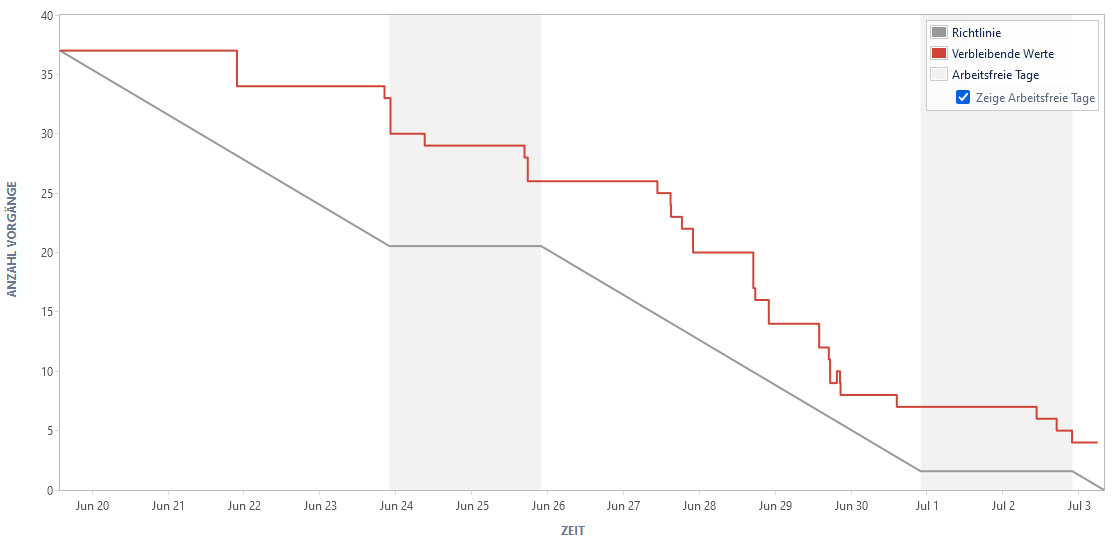
\includegraphics[height=0.5\textwidth]{images/burndown/sprint1vorg.png}
    \caption{Burndown-Diagramm: Release 3: Sprint 1 Vorgänge}
    \label{fig: sprint1vorg}
\end{figure}
Gegen Ende des Sprints am 19.06. wurde der Bug \hyperlink{S433}{STP23M-433} hinzugefügt. Dieser Vorgang ist allerdings schnell abgearbeitet worden und hatte keinen großen Einfluss auf den Sprint.

\subsubsection{Zeitschätzung}
Für alle Vorgänge des ersten Sprints gab es eine Zeitschätzung von insgesamt 90 Stunden und 15 Minuten. Tatsächlich benötigt wurden 105 Stunden und 33 Minuten. Dies ist eine Abweichung von circa 15 Stunden. Die Storys haben dabei allerdings weniger Zeit benötigt als geschätzt und die Aufgaben und Bugs mehr als geschätzt. Diese hohe Diskrepanz ist vor allem mit der Aufgabe \hyperlink{S418}{STP23M-418} zu erklären, welche 16 Stunden länger gedauert hat. 
\newpage
\section{Zweiter Sprint der dritten Veröffentlichung}
Die Bearbeitungsphase des zweiten Sprints verläuft vom 03.07.2023 bis zum 16.07.2023. Dabei findet bereits am 14.07. um 16 Uhr die Veröffentlichung statt. An den zwei darauffolgenden Tagen ist lediglich das Bearbeiten von Bugs zulässig. Der Umfang des Sprints ist noch vor dem Beginn durch das Hinzukommen von Bugs aus dem ersten Sprint erhöht worden. Zusätzlich sind die nicht beendete Aufgaben aus dem ersten Sprint hinzugekommen.

\subsection{User Storys}
Im Folgenden werden die User Storys des zweiten Sprints des dritten Releases beschrieben und es wird anschließend auf starke Abweichungen zwischen benötigter Zeit und geschätzter Zeit eingegangen. Eine Auflistung aller User Storys mit der jeweiligen benötigten Zeit und der jeweiligen geschätzten Zeit ist in der Tabelle~\ref{tab:story} zu finden. 
\subsubsection{Beschreibung der Storys}

Im Folgenden werden die Storys beschrieben. Dabei wird auf die erzielte beziehungsweise gewünschte Funktionalität eingegangen, die durch eine Aktion des Nutzers erfolgt.

\textbf{\hyperlink{T225}{\hypertarget{S225}{STP23M-225}}: Start an Encounter with a Wild Monster}

Der Nutzer begegnet einem wilden Monster in hohem Gras. Es wird dabei eine Ankündigung als Einleitung zum Kampf angezeigt, dass der Kampf in Kürze gestartet wird.

\textbf{\hyperlink{T226}{\hypertarget{S226}{STP23M-226}}: Switch to Encounter Scene Wild Monster}

Ziel dieser Story ist der Übergang zwischen dem Spielbildschirm und der Kampfszene beim Begegnen eines wilden Monsters zu implementieren. Die Ankündigung der Begegnung des wilden Monsters wird angezeigt. Der Nutzer drückt auf die Interaktionstaste und es wird zur Kampfszene gewechselt.

\textbf{\hyperlink{T233}{\hypertarget{S233}{STP23M-233}}: Current Monster Info Encounter}

Der Nutzer befindet sich in der Kampfszene und drückt auf den Knopf für die Monsterdetails des jetzigen Monsters. Es öffnet sich ein neues Fenster, in dem alle wichtigen Attribute und Details aufgezeigt werden.

\textbf{\hyperlink{T236}{\hypertarget{S236}{STP23M-236}}: Defeat opposing current monster}

Der Nutzer sieht die aktuellen Fähigkeiten von seinem jetzigen Monster und das gegnerische Monster hat aktuell niedrige Lebenspunkte. Der Nutzer setzt seinen Zug mit einer beliebigen Fähigkeit und besiegt dabei das gegnerische Monster. Dabei werden seine Lebenspunkte infolgedessen auf null gesetzt. Es erscheint daraufhin eine Benachrichtigung in dem Ereignisprotokoll. 

\textbf{\hyperlink{T237}{\hypertarget{S237}{STP23M-237}}: Level up Monster}

Diese Story ermöglicht dem Nutzer, den Levelaufstieg des eigenen Monsters zu betrachten und dabei die verbesserten Attribute zu sehen. Der Nutzer besiegt das gegnerische Monster und das jetzige Monster erhält Erfahrungspunkte, mit denen er im Level aufsteigen kann. Somit ist das Level hochinkrementiert und es öffnet sich ein Popup, in welchem die verbesserten Attribute dargestellt werden.

\textbf{\hyperlink{T238}{\hypertarget{S238}{STP23M-238}}: Win Encounter}

Als Folgerung dieser Story kann der Nutzer mithilfe seiner Monster einen Kampf gewinnen. Dabei wendet der Nutzer eine Fähigkeit seines jetzigen Monsters auf das gegnerische Monster an und besiegt es dabei. Der gegnerische Trainer hat keine anderen Monster mehr am Leben und somit gewinnt der Nutzer den Kampf. Es erscheint dabei ein Popup mit der Ankündigung über den Gewinn und das Textfeld wird dementsprechend aktualisiert. 

\textbf{\hyperlink{T239}{\hypertarget{S239}{STP23M-239}}: Switch to Ingame}

Der Nutzer hat die Ankündigung über den Gewinn oder den Verlust eines Kampfs erhalten. Die Ankündigung wird vom Nutzer durch Drücken des Knopfs 'OK' wahrgenommen und es wird in den Spielbildschirm gewechselt. 

\textbf{\hyperlink{T240}{\hypertarget{S240}{STP23M-240}}: Flee Popup Wild Monster}

Der Nutzer befindet sich in einem Kampf gegen ein wildes Monster und drückt den Knopf 'Fliehen'. Es erscheint ein Popup, in dem der Nutzer die Aktion bestätigen soll.

\textbf{\hyperlink{T241}{\hypertarget{S241}{STP23M-241}}: Flee Wild Monster}

Es wird ein Popup über die Bestätigung der 'Fliehen-Aktion' dargestellt. Der Nutzer nimmt die Flucht auf und der Kampf wird beendet. Der Nutzer gelangt nach wenigen Sekunden in den Spielbildschirm.

\textbf{\hyperlink{T243}{\hypertarget{S243}{STP23M-243}}: Show Active Team}

Der Spielbildschirm wird aktuell dargestellt. Der Nutzer drückt auf den Knopf 'Monster' und es öffnet sich ein neues Fenster, in dem das aktive Team an Monstern angezeigt wird.

\textbf{\hyperlink{T244}{\hypertarget{S244}{STP23M-244}}: Change Monster Order}

Der Nutzer sieht das Fenster des aktiven Teams an Monstern, das mindestens zwei Monster enthält. Der Nutzer drückt auf einen der Pfeilknöpfe. Dadurch ändert sich die Reihenfolge der Monster. 

\textbf{\hyperlink{T245}{\hypertarget{S245}{STP23M-245}}: Remove Monster Active Team}

Das Fenster des aktiven Teams an Monster wird dargestellt. Der Nutzer entfernt eines der Monster aus der Liste mit dem Knopf 'Aus dem Team entfernen'. Das gewählte Monster verschwindet aus der Liste und ein Popup öffnet sich, in dem die Aktion bestätigt wird. 

\textbf{\hyperlink{T246}{\hypertarget{S246}{STP23M-246}}: Show Other Monsters}

Der Nutzer sieht das Fenster des aktiven Teams. Dabei drückt er auf die Registerkarte 'Andere' und infolgedessen werden die anderen Monster des Nutzers angezeigt, die nicht zum aktiven Team gehören.

\textbf{\hyperlink{T247}{\hypertarget{S247}{STP23M-247}}: Monster Info}

Durch diese Story kann der Nutzer die Details eines gewünschten Monsters sehen. Der Nutzer sieht das aktive Team an Monstern und drückt auf den Knopf der Monsterdetails für ein beliebiges Monster. Es öffnet sich ein neues Fenster mit allen Attributen beziehungsweise Fähigkeiten, die das Monster besitzt.

\textbf{\hyperlink{T248}{\hypertarget{S248}{STP23M-248}}: Go Back from Details}

Die Monsterdetails werden in einem Fenster angezeigt. Der Nutzer kehrt zu der Monsterliste durch Drücken des Pfeilknopfs zurück. Somit wird die Monsterliste wieder dargestellt.

\textbf{\hyperlink{T249}{\hypertarget{S249}{STP23M-249}}: Add Monster to Active Team}

Der Nutzer sieht den Inhalt der Registerkarte 'Andere', also die im aktiven Team nicht anwesenden Monster. Der Nutzer drückt bei einem beliebigen Monster auf den Knopf 'Zum aktiven Team hinzufügen'. Das gewählte Monster verschwindet auf dieser Registerkarte und es öffnet sich ein Popup, in dem die Aktion bestätigt wird.

\textbf{\hyperlink{T250}{\hypertarget{S250}{STP23M-250}}: Limited Num of Monsters Active Team}

Der Inhalt der Registerkarte 'Andere' wird dargestellt. Das aktive Team an Monstern hat bereits eine Anzahl von sechs Monstern. Der Nutzer versucht ein beliebiges Monster zum aktiven Team hinzuzufügen. Es erscheint die Fehlermeldung, dass die gewünschte Aktion aufgrund der vollen Kapazität des aktiven Teams nicht erfolgt ist.

\textbf{\hyperlink{T256}{\hypertarget{S256}{STP23M-256}}: Show Keybindings}

Das Einstellungsmenü wird auf dem Bildschirm angezeigt. Der Nutzer drückt auf den Knopf 'Tastenkürzel' und damit werden die Einstellungen für die Tastenkürzel dargestellt.

\textbf{\hyperlink{T257}{\hypertarget{S257}{STP23M-257}}: Start Change Keybinding}

Der Nutzer drückt auf eine beliebige Taste, für die er das Kürzel ändern möchte. Es wird auf eine Eingabe vom Nutzer gewartet.

\textbf{\hyperlink{T258}{\hypertarget{S258}{STP23M-258}}: Finish Change Keybinding}

Es wird vom Nutzer eine Eingabe erwartet und der Nutzer drückt eine beliebige Taste auf seiner Tastatur. Die gedrückte Taste hat ein neues Kürzel und die Konfiguration wird gespeichert.

\textbf{\hyperlink{T259}{\hypertarget{S259}{STP23M-259}}: Change to Default Keybindings}

Der Nutzer sieht das Einstellungsfenster für die Tastenkürzel. Der Nutzer drückt auf den Knopf 'Standard' und dadurch werden alle Tastenkürzel zu den Standard-Tastenkürzeln zurückgesetzt.

\textbf{\hyperlink{T260}{\hypertarget{S260}{STP23M-260}}: Go Back from Keybindings}

Das Einstellungsfenster für die Tastenkürzel wird auf dem Bildschirm dargestellt. Der Nutzer drückt auf den Pfeilknopf und das aktuelle Fenster wird durch das Einstellungsmenü ersetzt.

\textbf{\hyperlink{T272}{\hypertarget{S272}{STP23M-272}}: 1v2 Battleground Situation}

Der Nutzer startet einen Kampf gegen zwei Trainer gleichzeitig. Es wird in die Kampfszene gewechselt und gegen den Nutzer spielen zwei Trainer mit ihren jeweiligen aktuellen Monstern. 

\textbf{\hyperlink{T273}{\hypertarget{S273}{STP23M-273}}: Opponent attack}

Die Kampfszene wird dargestellt und alle Spieler haben ihre Züge festgesetzt. Es wird die Fähigkeit des gegnerischen Monsters auf das aktuelle Monster des Nutzers angewandt und verliert somit Lebenspunkte. Das Ereignisprotokoll wird entsprechend aktualisiert.

\textbf{\hyperlink{T274}{\hypertarget{S274}{STP23M-274}}: Encounter lost}

Der Nutzer sieht die Kampfszene und sein aktuelles Monster weist sehr niedrige Lebenspunkte auf. Es wird die Fähigkeit des gegnerischen Monsters angewandt und der Nutzer verliert infolgedessen den Kampf. Ein Popup mit der Ankündigung, dass der Kampf verloren ist, erscheint.

\textbf{\hyperlink{T275}{\hypertarget{S275}{STP23M-275}}: 2v2 Battleground Situation}

Der Nutzer startet einen Kampf gegen zwei Trainer mit Unterstützung eines weiteren Trainers. Es wird in die Kampfszene gewechselt, welche eine Zwei-gegen-Zwei-Kampfszenario darstellt.

\textbf{\hyperlink{T276}{\hypertarget{S276}{STP23M-276}}: Show Change Monster Window}

Der Nutzer sieht die Kampfszene und hat seinen Zug noch nicht festgesetzt. Der Nutzer drückt auf den Knopf 'Monster auswechseln' und es öffnet sich ein Fenster für den Monsterwechsel.

\textbf{\hyperlink{T277}{\hypertarget{S277}{STP23M-277}}: Change Current Monster}

Das Fenster für den Monsterwechsel wird dargestellt. Der Nutzer wechselt das jetzige Monster durch ein beliebiges Monster aus der Liste aus, indem er 'Zu diesem Monster wechseln' drückt. Das jetzige Monster wird durch das gewählte Monster ausgewechselt.

\textbf{\hyperlink{T279}{\hypertarget{S279}{STP23M-279}}: Level up Monster New Ability}

Die Kampfszene wird dargestellt. Der Nutzer besiegt hierbei das gegnerische Monster und das jetzige Monster erhält Erfahrungspunkte, mit denen es im Level aufsteigen kann. Somit ist das Level hochinkrementiert und es öffnet sich ein Popup, in dem die verbesserten Attribute und eine neu erlernte Fähigkeit für das jetzige Monster angezeigt werden.
\subsubsection{Bewertung der Storys}

Im Folgenden werden die Storys bewertet, die eine starke Abweichung zwischen der benötigten Zeit und der geschätzten Zeit aufweisen.

\textbf{\hyperlink{T225}{\hypertarget{S225}{STP23M-225}}: Start an Encounter with a Wild Monster}

Das Starten eines Kampfes gegen ein wildes Monster beträgt als Story einen Story Point und somit wurde sie mit einer Stunde geschätzt. Da die Funktionalität des Kampfstarts bereits in \hyperlink{T223}{\hypertarget{S223}{STP23M-223}} implementiert wurde, konnte diese Story innerhalb von fünf Minuten abgeschlossen werden.

\textbf{\hyperlink{T226}{\hypertarget{S226}{STP23M-226}}: Switch to Encounter Scene Wild Monster}

Diese Story hat drei Story Points und beträgt somit geschätzt drei Stunden. Allerdings konnte die Story innerhalb von 30 Minuten erledigt werden, da die meisten Funktionen bereits in der implementierten Story \hyperlink{T224}{\hypertarget{S224}{STP23M-224}} vorhanden waren.

\textbf{\hyperlink{T243}{\hypertarget{S243}{STP23M-243}}: Show Active Team}

Das Anzeigen des aktiven Teams wurde als Story mit zwei Story Points geschätzt und beträgt somit geschätzt zwei Stunden. Dennoch wurde die Story aufgrund des schwierigen Designs innerhalb von drei Stunden und 30 Minuten erledigt werden, sodass das Fenster mit den Mockups nahezu übereinstimmend ist. 

\textbf{\hyperlink{T244}{\hypertarget{S244}{STP23M-244}}: Change Monster Order}

Diese Story hat zwei Story Points und beträgt also geschätzt zwei Stunden. Der Entwickler konnte die Story in 15 Minuten erledigen, da die Grundfunktionalität bereits bestehend war und nur die Serverabfrage implementiert werden musste.

\textbf{\hyperlink{T245}{\hypertarget{S245}{STP23M-245}}: Remove Monster Active Team}

Die Story hat zwei Story Points und beträgt somit geschätzt zwei Stunden. Dennoch konnte die Story analog zu der Story \hyperlink{T244}{\hypertarget{S244}{STP23M-244}} implementiert werden, sodass die Story in nur 15 Minuten erledigt werden konnte. 

\textbf{\hyperlink{T256}{\hypertarget{S256}{STP23M-256}}: Show Keybindings}

Das Anzeigen der Tastenkürzel wurde als Story mit zwei Story Points geschätzt und beträgt somit geschätzt zwei Stunden. Das genaue Design der Einstellungen war allerdings schwierig umzusetzen, sodass die Story drei Stunden und 20 Minuten an Arbeitsaufwand benötigte.

\textbf{\hyperlink{T257}{\hypertarget{S257}{STP23M-257}}: Start Change Keybinding}

Diese Story hat einen Story Point und beträgt somit geschätzt eine Stunde. Dennoch konnte sie der Entwickler in sieben Stunden und 50 Minuten erledigen. Der Grund beruht darauf, dass am Anfang des Implementierens ein falscher Ansatz verfolgt worden ist, der im Nachhinein von dem Entwickler verbessert und vervollständigt wurde. 

\textbf{\hyperlink{T272}{\hypertarget{S272}{STP23M-272}}: 1v2 Battleground Situation}

Die Story hat fünf Story Points und beträgt somit geschätzt fünf Stunden. Allerdings konnte die Story innerhalb von sieben Stunden erledigt werden. Das liegt daran, dass das Sicherstellen der erzielten Funktionalität mehr Zeit in Anspruch genommen hat.

\textbf{\hyperlink{T273}{\hypertarget{S273}{STP23M-273}}: Opponent attack}

Das Anzeigen der Angriffe der Gegner wurde als Story mit zwei Story Points geschätzt und beträgt somit geschätzt zwei Stunden. Dennoch konnte die Story innerhalb von 15 Minuten erledigt werden, da die Grundfunktionalität für das Anzeigen bereits in der Story \hyperlink{T235}{\hypertarget{S235}{STP23M-235}} implementiert wurde.

\textbf{\hyperlink{T223}{\hypertarget{S223}{STP23M-223}}: Start an Encounter with a Trainer}

Diese Story wurde aus dem ersten Sprint in den zweiten Sprint aufgrund von Zeitproblemen verschoben. Sie wurde mit einem Story Point und somit mit einer Stunde geschätzt. Allerdings konnte die Story innerhalb von einem Arbeitstag und zwei Stunden erledigt werden, da das Finden eines optimalen Ansatzes mehr Zeit als erwartet benötigt hat. Auf diese Weise konnte die Funktionalität sichergestellt werden.  

\textbf{\hyperlink{T235}{\hypertarget{S235}{STP23M-235}}: Use an Ability}

Die Story ist auch aus dem ersten Sprint übertragen worden. Sie wurde mit vier Story Points und mit vier Stunden geschätzt. Der Entwickler konnte die Story allerdings in sechs Stunden und 30 Minuten abschließen. Das ist darauf zurückzuführen, dass die Recherche und das Implementieren des Ansatzes mehr Zeit in Anspruch genommen hatte. 

\textbf{\hyperlink{T236}{\hypertarget{S236}{STP23M-236}}: Defeat opposing current monster}

Das Besiegen des gegnerischen jetzigen Monsters wurde als Story mit zwei Story Points und zwei Stunden geschätzt. Die Story konnte allerdings nicht in dem zweiten Sprint abgeschlossen werden, da viele Zeitprobleme und Abhängigkeiten zwischen den Storys vor dem Releaseende bestanden haben, sodass sie in das nächste Release übernommen werden mussten.

\textbf{\hyperlink{T277}{\hypertarget{S277}{STP23M-277}}: Change Current Monster}

Diese Story hat zwei Story Points und beträgt somit geschätzt zwei Stunden. Es herrschte aber vor dem Releaseende Zeitdruck und Abhängigkeiten zwischen den einzelnen Storys, sodass sie nicht innerhalb des Zeitraums des Releases erledigt werden konnte. Die Story wird dementsprechend in das nächste Release übernommen.
\subsection{Aufgaben und Bugs}
Im zweiten Sprint enthälz erneut neben den Storys Aufgaben und Bugs. Dabei gibt es fünf Aufgaben und sechs Bugs. Bei den Bugs handelt es sich zum größten Teil um Fehler, die im ersten Sprint dazugekommen sind. Die Aufgaben sollen technische Anforderungen und die Internationalisierung sicherstellen.
Eine Auflistung aller Aufgaben und Bugs ist in der Tabelle \ref{tab:task1} zu finden.

\subsubsection{Beschreibung der Aufgaben und Bugs}
Im Folgenden werden sämtliche Aufgaben und Bugs des zweiten Sprints beschrieben. Es wird dabei auf ihre Einzelheiten eingegangen.

\textbf{\hyperlink{T425}{\hypertarget{S425}{STP23M-425}}: Test Coverage sicherstellen}
\newline
\newline
Durch diese Aufgabe soll sichergestellt werden, dass die geforderten 70 \% Testcoverage erreicht werden. Zusätzlich soll ein Test \textit{Critical Path V3} erstellt werden, der die Anforderungen der dritten Veröffentlichung in einem Test hintereinander testet, um die Funktionalität der Anwendung sicherzustellen.
\newline
\newline
\textbf{\hyperlink{T427}{\hypertarget{S427}{STP23M-427}}: Kampf wiederherstellen}
\newline
\newline
Eine Anforderung des Kunden für das dritte Release lautet, dass es problemlos möglich sein soll, die Anwendung in einem Kampf oder Ähnlichem zu verlassen und wiederzubetreten. Diese Aufgabe soll diese Anforderung sicherstellen, sodass sich beim erneuten Starten der Anwendung der Nutzer wieder im Kampf befindet.
\newline
\newline
\textbf{\hyperlink{T430}{\hypertarget{S430}{STP23M-430}}: Chinesische Übersetzung}
\newline
\newline
Seit dem zweiten Release ist die Anwendung in verschiedenen Sprachen spielbar. Da im Team eine Person vertraut mit der chinesischen Sprache ist, dient diese Aufgabe dazu, dieser Person die Zeit zu geben, alle Texte in das Chinesische zu übersetzen.
\newline
\newline
\textbf{\hyperlink{T431}{\hypertarget{S431}{STP23M-431}}: Refactor vor dem Release}
\newline
\newline
Diese Aufgabe soll gegen Ende des zweiten Sprints bearbeitet werden. Dabei soll der Code auf unnötige Imports und Variablen, Felder oder Ähnliches überprüft werden. Diese sollen dann entfernt werden. Zusätzlich soll versucht werden, alle Warnungen zu entfernen. Ein weiteres Ziel der Aufgabe ist es sicherzustellen, dass der gesamte Code korrekt eingerückt ist, um eine gute Lesbarkeit zu garantieren.
\newline
\newline
\textbf{\hyperlink{T432}{\hypertarget{S432}{STP23M-432}}: Benachrichtigung auf dem Handy nach jedem Gebietswechsel}
\newline
\newline
Bei dieser Aufgabe handelt es sich um ein Bugticket. Dieser Bug existiert, seitdem das Benachrichtigungs- bzw. Hilfesystem implementiert wurde. Durch diesen Task soll der Fehler behoben werden, dass die Hilfenachrichten vor dem Erhalt des ersten Monsters immer wieder angezeigt werden. Diese werden erneut angezeigt, obwohl die Benachrichtigung bereits gelesen wurde. Dies geschieht, sobald das Areal gewechselt wird oder das Spiel erneut gestartet wird.
\newline
\newline
\textbf{\hyperlink{T434}{\hypertarget{S434}{STP23M-434}}: Audioeinstellung wird nicht nach Szenenwechsel gesetzt}
\newline
\newline
Für das Bonusfeature Musik wurde zusätzlich die Möglichkeit geschaffen, die Musik stumm zu stellen beziehungsweise die Lautstärke einzustellen. Beim Wechseln der Szene wird allerdings die Musik wieder auf die Standardlautstärke zurückgesetzt. Zum Beispiel wird beim Übergang vom Hauptmenü zur Trainererstellung die Musik wieder laut, nachdem sie im Hauptmenü stumm geschaltet wurde. Bei dieser Aufgabe handelt es sich also um einen Bug.
\newline
\newline
\textbf{\hyperlink{T435}{\hypertarget{S435}{STP23M-435}}: Audioeinstellungsschieber zeigt die aktuelle Lautstärke nicht an}
\newline
\newline
Hier handelt es sich ebenfalls um einen Bug. So wird beim Öffnen der Audioeinstellung nicht die aktuelle Lautstärke angezeigt, sondern der Schieber steht zu Beginn komplett links auf Stumm. Diese Aufgabe soll den Fehler beheben, sodass beim Öffnen die aktuelle Lautstärke angezeigt wird.
\newline
\newline
\textbf{\hyperlink{T436}{\hypertarget{S436}{STP23M-436}}: Neue Dialoge}
\newline
\newline
Nach einem Server Patch sind weitere Bereiche mit neuen NPCs hinzugekommen. Nachdem im ersten Sprint alle vorhandenen NPCs mit eigenen Dialogen versehen worden sind, müssen die neuen NPCs mit eigenen Texten versehen werden. Das soll in dieser Aufgabe geschehen.
\newline
\newline
\textbf{\hyperlink{T437}{\hypertarget{S437}{STP23M-437}}: Die Region Encounter Test ist nicht betretbar}
\newline
\newline
Seit dem Server Update 3.0.0 gibt es neben der Region 'Albertania' die weitere Region 'Encounter Test'. Diese Region dient dem Testen der 'Encounter'. Bei dem Versuch die Region zu betreten, kommt es in der Anwendung zu einem Fehler und der Bildschirm bleibt schwarz. Dieses Bugticket soll den Fehler beheben und die 'Encounter Test' Region betretbar machen.
\newline
\newline
\textbf{\hyperlink{T438}{\hypertarget{S438}{STP23M-438}}: Es werden nicht alle Areale korrekt geladen}
\newline
\newline
Dies ist noch ein Bug, welcher seit dem Implementieren des Renderns der Gebiete besteht. In einigen Gebieten gibt es schwarze Flächen, die nicht richtig geladen werden. Nach dem Bearbeiten dieses Bugtickets sollen alle Gebiete korrekt angezeigt werden.
\newline
\newline
\textbf{\hyperlink{T439}{\hypertarget{S439}{STP23M-439}}: Fliehen funktioniert nicht nach dem Klicken auf die Fähigkeiten}
\newline
\newline
Bei diesem Vorgang handelt es sich um einen Bug. Beim Testen der Funktionalität Fähigkeiten auszuführen ist aufgefallen, dass danach der 'Fliehenknopf' nicht mehr funktioniert. Dieses Problem soll mit diesem Bugvorgang behoben werden.
\newline
\newline
\textbf{\hyperlink{T478}{\hypertarget{S478}{STP23M-478}}: General bug fixes}
\newline
\newline
Dieser Bug ist nach der Veröffentlichung dazugekommen. Hier sollen verschiedene Fehler behoben werden, die nach dem letzten Merge hinzugekommen sind. Dieser konnte aufgrund von Zeitmangel nicht ausgiebig getestet werden.
\newline
\newline
\textbf{\hyperlink{T479}{\hypertarget{S479}{STP23M-479}}: Lebenswert in der Encounter aktualisieren}
\newline
\newline
Hierbei handelt es sich ebenfalls um einen Bug, welcher nach der Veröffentlichung dazugekommen ist. Dieses Bugticket soll speziell den Fehler beheben, dass die Lebensanzeige nicht korrekt aktualisiert wird.
\newline
\newline
\textbf{\hyperlink{T480}{\hypertarget{480}{STP23M-480}}: Problem beim Encounter verlassen}
\newline
\newline
Auch dieser Bug ist nach der Veröffentlichung hinzugefügt worden. Seit dem letzten Merge gibt es Probleme beim Verlassen eines Kampfes. Dieser Vorgang soll dieses Problem beheben.
\subsubsection{Bewertung der Aufgaben und Bugs}
Die meisten Aufgaben und Bugs wurden innerhalb der geschätzten Zeit bearbeitet. Lediglich die Aufgaben \hyperlink{S425}{STP23M-425} und \hyperlink{S436}{STP23M-436} haben eine längere Zeit als geschätzt in Anspruch genommen. Mit einer Stunde beziehungsweise zwei Stunden und 30 Minuten hält sich der Mehraufwand dabei in Grenzen. Einige Aufgaben wie zum Beispiel \hyperlink{S430}{STP23M-430} wurden sogar schneller bearbeitet als geschätzt. Die meisten Aufgaben und Bugs wurden allerdings genau in der geschätzten Zeit bearbeitet. Leider gibt es mit dem Bug \hyperlink{S432}{STP23M-432} auch einen Vorgang unter den Aufgaben und Bugs, der nicht bearbeitet wurde. Der zuständige Entwickler hat keinen Lösungsansatz für den Fehler gefunden. \\
Abschließend kann positiv erwähnt werden, dass die geschätzte Zeit nahezu identisch mit der tatsächlich gebrauchten Zeit ist. Lediglich der nicht bearbeitete Bug stellt ein negativer Punkt in der Bewertung der Aufgaben und Bugs dar.
\subsection{Bewertung des Sprints}
Im zweiten Sprint wurde ein Aspekt der Anwendung überarbeitet und es sind weiter Features dazugekommen. Bei dem überarbeiteten Feature handelt es sich um die Monsterliste. Hinzugekommen ist das Bonusfeature, welches das Bearbeiten der Steuerung durch den Nutzer ermöglichen soll. Des Weiteren wurde das komplette Kampfgeschehen implementiert, sodass alle Kampfsituationen durchgeführt und angezeigt werden können.  Zusätzlich gab es einige technische Anforderungen, die sichergestellt werden mussten. Die Internationalisierung ist ein Bonusfeature aus der zweiten Veröffentlichung und musste ebenfalls sichergestellt werden.\\
\begin{figure}[H]
    \center
    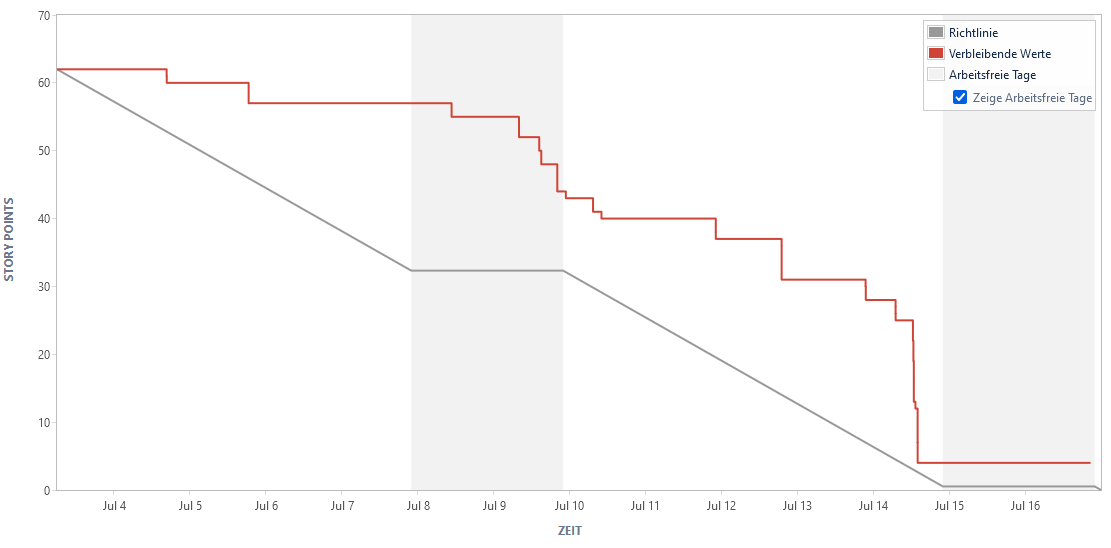
\includegraphics[height=0.5\textwidth]{images/burndown/sprint2Story.png}
    \caption{Burndown-Diagramm: Release 3: Sprint 2 Story Points}
    \label{fig: sprint2Story}
\end{figure}

Wie schon im ersten Sprint wurden im zweiten Sprint ebenfalls nicht alle Storys abgeschlossen. Wie in der Abbildung \ref{fig: sprint2Story} zu sehen ist, hängt dies mit zwei Phasen des Sprints zusammen. So wurde bis zum Wochenende der ersten Woche nicht sehr viele Storys abgearbeitet. Am Wochenende ist dann zwar ein guter Fortschritt erzielt worden, der Rückstand konnte aber nicht komplett aufgeholt werden. Auch zu Beginn der zweiten Woche gab es wieder wenig Fortschritt, was die zweite schlechte Phase darstellt. Zwar wurde am Freitag versucht, alle Anforderungen zu implementieren, aber der Rückstand war zu groß. Dabei sind zwei Storys und ein Bug nicht abgeschlossen worden. Die Storys \hyperlink{S236}{STP23M-236} und \hyperlink{S277}{STP23M-277} wurden aufgrund von Zeitmangel am Freitag nicht mehr fertiggestellt. Für den Bug \hyperlink{S432}{STP23M-432} wurde keine Lösung gefunden. \\ Die Bewertung kann, aufgrund der nicht abgeschlossenen Vorgänge, nicht positiv ausfallen. So müssen und werden die fehlenden Anforderungen in der vierten Veröffentlichung nachgereicht. Auch die geforderten 70\% Test Coverage wurde mit 64.17\% nicht erreicht. Auch diese wird in der vierten Veröffentlichung verbessert werden müssen.

\subsubsection{Erhöhung der Vorgänge}
Im zweiten Sprint der dritten Veröffentlichung gab es fünf Umfangsänderungen.
\begin{figure}[H]
    \center
    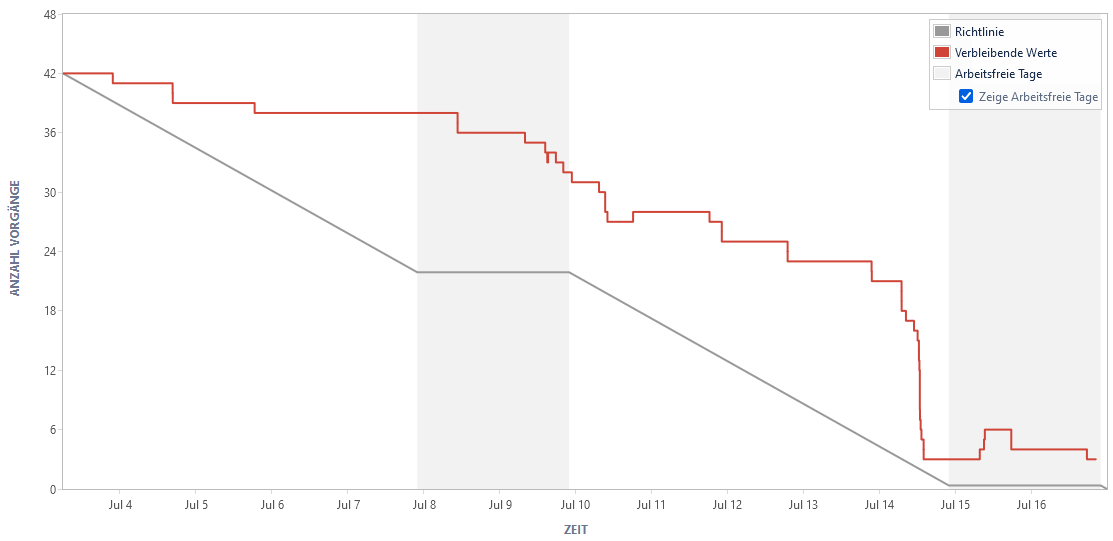
\includegraphics[height=0.5\textwidth]{images/burndown/sprint2vorg.png}
    \caption{Burndown-Diagramm: Release 3: Sprint 2 Vorgänge}
    \label{fig: sprint2vorg}
\end{figure}

In der ersten Woche des Sprints ist der Bug \hyperlink{S439}{STP23M-439} hinzugekommen. Dieser wurde schnell bearbeitet. In der zweiten Woche vor der Veröffentlichung am Freitag ist der Bug \hyperlink{S438}{STP23M-438} dazugekommen, der nicht direkt bearbeitet wurde. Am Wochenende nach der Veröffentlichung sind mit \hyperlink{S478}{STP23M-478}, \hyperlink{S479}{STP23M-479} und \hyperlink{S480}{STP23M-480} drei weitere Bugs dazugekommen. Die letzten beiden wurden schnell abgearbeitet. Lediglich \hyperlink{S478}{STP23M-478} wurde erst am Sonntag geschlossen.

\subsubsection{Zeitschätzung}
Die Zeitschätzung für alle Vorgänge des zweiten Sprints betrug 91 Stunden und 40 Minuten. Die tatsächliche benötigte Zeit betrug jedoch 94 Stunden und 35 Minuten. Die Abweichung beträgt demnach nur circa drei Stunden, was im Vergleich zum ersten Sprint mit circa 15 Stunden zunächst positiv erscheint. Allerdings wurden, wie oben beschreiben, die Storys \hyperlink{S236}{STP23M-236} und \hyperlink{S277}{STP23M-277} und der Bug \hyperlink{S432}{STP23M-432} nicht abgeschlossen, wodurch hier keine positive Bewertung gegeben werden kann. 